%%---------------------------------------------------------------------------------%%
%% knitr files for the supplementary material to the paper "Nested effects modelling of Wnt signalling predicts the sensitization of cancer cells to Wnt ligands in colorectal cancer."
%% Giusi Moffa
%% University of Regensburg
%
%% Last modified: July 16, 2014
%
%% Disclaimer: The code in this archive is not guaranteed to be optimised or free of bugs.
%% Please report any issues to the authors (giusi.moffa@ur.de).
%%---------------------------------------------------------------------------------%%


%%% From within the working folder run the following
%%% library(knitr)
% purl("wntSupp.Rnw") ## to extract the code
% knit('wntSupp.Rnw')

\documentclass[a4paper]{article}\usepackage[]{graphicx}\usepackage[]{color}
%% maxwidth is the original width if it is less than linewidth
%% otherwise use linewidth (to make sure the graphics do not exceed the margin)
\makeatletter
\def\maxwidth{ %
  \ifdim\Gin@nat@width>\linewidth
    \linewidth
  \else
    \Gin@nat@width
  \fi
}
\makeatother

\definecolor{fgcolor}{rgb}{0.345, 0.345, 0.345}
\newcommand{\hlnum}[1]{\textcolor[rgb]{0.686,0.059,0.569}{#1}}%
\newcommand{\hlstr}[1]{\textcolor[rgb]{0.192,0.494,0.8}{#1}}%
\newcommand{\hlcom}[1]{\textcolor[rgb]{0.678,0.584,0.686}{\textit{#1}}}%
\newcommand{\hlopt}[1]{\textcolor[rgb]{0,0,0}{#1}}%
\newcommand{\hlstd}[1]{\textcolor[rgb]{0.345,0.345,0.345}{#1}}%
\newcommand{\hlkwa}[1]{\textcolor[rgb]{0.161,0.373,0.58}{\textbf{#1}}}%
\newcommand{\hlkwb}[1]{\textcolor[rgb]{0.69,0.353,0.396}{#1}}%
\newcommand{\hlkwc}[1]{\textcolor[rgb]{0.333,0.667,0.333}{#1}}%
\newcommand{\hlkwd}[1]{\textcolor[rgb]{0.737,0.353,0.396}{\textbf{#1}}}%

\usepackage{framed}
\makeatletter
\newenvironment{kframe}{%
 \def\at@end@of@kframe{}%
 \ifinner\ifhmode%
  \def\at@end@of@kframe{\end{minipage}}%
  \begin{minipage}{\columnwidth}%
 \fi\fi%
 \def\FrameCommand##1{\hskip\@totalleftmargin \hskip-\fboxsep
 \colorbox{shadecolor}{##1}\hskip-\fboxsep
     % There is no \\@totalrightmargin, so:
     \hskip-\linewidth \hskip-\@totalleftmargin \hskip\columnwidth}%
 \MakeFramed {\advance\hsize-\width
   \@totalleftmargin\z@ \linewidth\hsize
   \@setminipage}}%
 {\par\unskip\endMakeFramed%
 \at@end@of@kframe}
\makeatother

\definecolor{shadecolor}{rgb}{.97, .97, .97}
\definecolor{messagecolor}{rgb}{0, 0, 0}
\definecolor{warningcolor}{rgb}{1, 0, 1}
\definecolor{errorcolor}{rgb}{1, 0, 0}
\newenvironment{knitrout}{}{} % an empty environment to be redefined in TeX

\usepackage{alltt}


\usepackage{a4wide}
\usepackage{amsmath, amsfonts, amssymb}
\usepackage{color}
\usepackage{natbib}
\IfFileExists{upquote.sty}{\usepackage{upquote}}{}
\begin{document}
\setkeys{Gin}{width=.9\textwidth}
%opts_chunk$set(eval=FALSE)

\title{Bayesian model comparison of nested effect models for Wnt signalling analysis \\
{\small Supplement to ``Nested effects modelling of Wnt signalling suggests the sensitization of cancer cells to Wnt ligands in colorectal cancer''.}}
%\subtitle{Supplement to ``Wnt secretion is required for colon cancer cell survival''}
\author{Giusi Moffa}
\date{}

\maketitle

%%%----------------------------------------------------------%%%
%%%--------- Input data analysis file----------%%%

%%---------------------------------------------------------------------------------%%
%% knitr files for the supplementary material to the paper "Nested effects modelling of Wnt signalling predicts the sensitization of cancer cells to Wnt ligands in colorectal cancer."
%% Giusi Moffa
%% University of Regensburg
%
%% Last modified: July 16, 2014
%
%% Disclaimer: The code in this archive is not guaranteed to be optimised or free of bugs.
%% Please report any issues to the authors (giusi.moffa@ur.de).
%%---------------------------------------------------------------------------------%%


%opts_chunk$set(cache=TRUE)
\begin{knitrout}
\definecolor{shadecolor}{rgb}{0.969, 0.969, 0.969}\color{fgcolor}\begin{kframe}
\begin{alltt}
\hlcom{# global chunk options}
\hlstd{opts_chunk}\hlopt{$}\hlkwd{set}\hlstd{(}\hlkwc{cache} \hlstd{=} \hlnum{FALSE}\hlstd{,} \hlkwc{autodep} \hlstd{=} \hlnum{TRUE}\hlstd{)}
\end{alltt}
\end{kframe}
\end{knitrout}

%opts_chunk$set(eval=FALSE) %%% somehow it does not seem to be inherited from the parent file
\section*{NEM analysis of WNT reads}
In the following we provide the code for the complete analysis, which were run under R version \verb'3.0.0' (nem version \verb'2.36.0', limma version \verb'3.16.1').

Record session information.
\begin{knitrout}
\definecolor{shadecolor}{rgb}{0.969, 0.969, 0.969}\color{fgcolor}\begin{kframe}
\begin{alltt}
\hlkwd{sessionInfo}\hlstd{()}
\end{alltt}
\begin{verbatim}
## R version 3.0.3 (2014-03-06)
## Platform: x86_64-apple-darwin10.8.0 (64-bit)
## 
## locale:
## [1] en_GB.UTF-8/en_GB.UTF-8/en_GB.UTF-8/C/en_GB.UTF-8/en_GB.UTF-8
## 
## attached base packages:
## [1] stats     graphics  grDevices utils     datasets  methods   base     
## 
## other attached packages:
## [1] knitr_1.6
## 
## loaded via a namespace (and not attached):
## [1] evaluate_0.5.5 formatR_0.10   highr_0.3      stringr_0.6.2 
## [5] tools_3.0.3
\end{verbatim}
\end{kframe}
\end{knitrout}

Install packages
\begin{knitrout}
\definecolor{shadecolor}{rgb}{0.969, 0.969, 0.969}\color{fgcolor}\begin{kframe}
\begin{alltt}
\hlkwd{source}\hlstd{(}\hlstr{"http://bioconductor.org/biocLite.R"}\hlstd{)}
\hlkwd{biocLite}\hlstd{(}\hlstr{"Rgraphviz"}\hlstd{,} \hlkwc{type} \hlstd{=} \hlstr{"source"}\hlstd{)}
\hlkwd{biocLite}\hlstd{(}\hlstr{"edgeR"}\hlstd{)}
\hlkwd{library}\hlstd{(edgeR)}
\end{alltt}
\end{kframe}
\end{knitrout}

\subsubsection*{Data}
The reads obtained by RNA-Sequencing are read into R and normalised through the \verb'voom' function \cite{art:Smyth2014} of the \verb'limma' package. As it is standard practice the columns of the data matrix correspond to samples and the rows to genes. The data as normalised by \verb'voom' is then further processed for differential expression analysis with \verb'limma'.

\subsubsection*{Loading data}
From within the working folder, containing files \verb'wntCounts.RData' and \verb'wntExonLen.RData'.

\begin{knitrout}
\definecolor{shadecolor}{rgb}{0.969, 0.969, 0.969}\color{fgcolor}\begin{kframe}
\begin{alltt}
\hlkwd{load}\hlstd{(}\hlstr{"wntCounts.RData"}\hlstd{)}  \hlcom{### contains a variable D.counts with the the count data}
\hlkwd{load}\hlstd{(}\hlstr{"wntExonLen.RData"}\hlstd{)}  \hlcom{### contains a variable Dlength with the gene exon lengths}
\end{alltt}
\end{kframe}
\end{knitrout}

\subsubsection*{Remove short genes}
Genes shorter than 150bp are removed from the analysis since these should not be theoretically present, and eventual reads probably only happen by contamination.
%{\color{blue} Six genes are lost when looking at exons, probably due to different annotations, should these be kept in the analysis?}



\subsubsection*{Select only the replicates which passed the quality control filter}

\begin{knitrout}
\definecolor{shadecolor}{rgb}{0.969, 0.969, 0.969}\color{fgcolor}\begin{kframe}
\begin{alltt}
\hlstd{DsubNames} \hlkwb{<-} \hlkwd{grep}\hlstd{(}\hlstr{"_1|_2"}\hlstd{,} \hlkwd{colnames}\hlstd{(D2analysis),} \hlkwc{value} \hlstd{=} \hlnum{TRUE}\hlstd{)}
\hlstd{DsubNames} \hlkwb{<-} \hlstd{DsubNames[}\hlopt{-}\hlkwd{c}\hlstd{(}\hlnum{14}\hlopt{:}\hlnum{18}\hlstd{)]}
\hlstd{DsubNames}
\hlstd{DsubJ} \hlkwb{<-} \hlstd{D2analysis[, DsubNames]}
\hlkwd{colnames}\hlstd{(DsubJ)}
\hlkwd{dim}\hlstd{(DsubJ)}
\hlcom{# barplot(colSums(DsubJ)*1e-6, names=seq_along(length(DsubNames)))}
\end{alltt}
\end{kframe}
\end{knitrout}

\subsubsection*{Data transformation via voom}
Transform the data with voom to then apply the limma pipeline for differential analysis.

\begin{knitrout}
\definecolor{shadecolor}{rgb}{0.969, 0.969, 0.969}\color{fgcolor}\begin{kframe}
\begin{alltt}
\hlkwd{library}\hlstd{(limma)}
\hlkwd{library}\hlstd{(edgeR)}
\hlstd{isexpr} \hlkwb{<-} \hlkwd{rowSums}\hlstd{(}\hlkwd{cpm}\hlstd{(DsubJ)} \hlopt{>} \hlnum{1}\hlstd{)} \hlopt{>=} \hlnum{1}
\hlcom{## keep only genes with at least one count per million reads in at least one}
\hlcom{## sample (Note that cpm are not integers)}

\hlcom{## cpmD <- cpm(DsubJ) cpmDbool <- cpmD[which(rowSums(cpmD>1) >= 1),]}
\hlcom{## min(rowSums(cpmDbool))}

\hlstd{Dsel} \hlkwb{<-} \hlstd{DsubJ[isexpr, ]}
\hlkwd{colnames}\hlstd{(Dsel)} \hlkwb{<-} \hlkwd{colnames}\hlstd{(DsubJ)}
\hlkwd{dim}\hlstd{(Dsel)}
\hlstd{pickNames} \hlkwb{<-} \hlkwa{function}\hlstd{(}\hlkwc{x}\hlstd{)} \hlkwd{head}\hlstd{(}\hlkwd{unlist}\hlstd{(}\hlkwd{strsplit}\hlstd{(x,} \hlkwc{split} \hlstd{=} \hlstr{"_"}\hlstd{)),} \hlnum{1}\hlstd{)}
\hlstd{exps} \hlkwb{<-} \hlkwd{factor}\hlstd{(}\hlkwd{unname}\hlstd{(}\hlkwd{sapply}\hlstd{(}\hlkwd{colnames}\hlstd{(Dsel), pickNames)))}
\hlstd{design} \hlkwb{<-} \hlkwd{model.matrix}\hlstd{(}\hlopt{~}\hlnum{0} \hlopt{+} \hlstd{exps)}
\hlkwd{colnames}\hlstd{(design)} \hlkwb{<-} \hlkwd{make.names}\hlstd{(}\hlkwd{gsub}\hlstd{(}\hlstr{"exps"}\hlstd{,} \hlstr{""}\hlstd{,} \hlkwd{colnames}\hlstd{(design)))}
\hlcom{# image(t(apply(t(design), 1, rev)) ) # graphical visualization of design}
\hlcom{# matrix}
\hlkwd{colnames}\hlstd{(Dsel)} \hlkwb{<-} \hlkwd{unname}\hlstd{(}\hlkwd{sapply}\hlstd{(}\hlkwd{colnames}\hlstd{(Dsel), pickNames))}
\end{alltt}
\end{kframe}
\end{knitrout}

\begin{knitrout}
\definecolor{shadecolor}{rgb}{0.969, 0.969, 0.969}\color{fgcolor}\begin{kframe}
\begin{alltt}
\hlstd{D4nem} \hlkwb{<-} \hlkwd{voom}\hlstd{(Dsel, design,} \hlkwc{plot} \hlstd{=} \hlnum{TRUE}\hlstd{)}
\end{alltt}
\end{kframe}
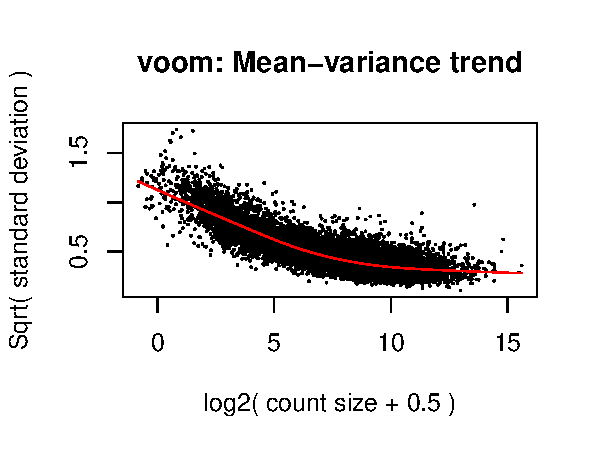
\includegraphics[width=\maxwidth]{figure/voomTransform} 

\end{knitrout}

%\clearpage

\subsection*{Definition of some functions which are used in the main procedure}
Define a number of functions so that the same processing can be more easily applied to different selections of experiments to model.

\subsubsection*{Function to perform the differential analysis via limma} 
Among other statistics posterior probabilities that genes are affected by certain perturbations are provided as output. The routine comes from the package \verb'limma' and is based on the Bayesian methods described in \cite{art:Smyth2004}. The parameter \verb'pr' gives the assumed prior probability of differential expression. In our analysis below we will set this parameter to .004, meaning that 4 genes in a thousand are a priori assumed to be differentially expressed. The prior reflects expert knowledge in that it was set in a way that the length of identified target lists roughly matches reports found in the literature.
\\
% 
\begin{knitrout}
\definecolor{shadecolor}{rgb}{0.969, 0.969, 0.969}\color{fgcolor}\begin{kframe}
\begin{alltt}
\hlstd{applyLimma} \hlkwb{<-} \hlkwa{function}\hlstd{(}\hlkwc{jdata}\hlstd{,} \hlkwc{ctrl}\hlstd{,} \hlkwc{pr} \hlstd{=} \hlnum{0.01}\hlstd{) \{}
    \hlkwd{require}\hlstd{(limma)}
    \hlstd{cn} \hlkwb{<-} \hlkwd{colnames}\hlstd{(jdata)}
    \hlcom{# colnames(jdata) <- make.names(cn)}
    \hlstd{exps} \hlkwb{<-} \hlkwd{factor}\hlstd{(}\hlkwd{colnames}\hlstd{(jdata))}
    \hlstd{design} \hlkwb{<-} \hlkwd{model.matrix}\hlstd{(}\hlopt{~}\hlnum{0} \hlopt{+} \hlstd{exps)}
    \hlkwd{colnames}\hlstd{(design)} \hlkwb{<-} \hlkwd{unique}\hlstd{(cn)}
    \hlstd{cn} \hlkwb{<-} \hlkwd{setdiff}\hlstd{(cn, ctrl)}
    \hlstd{fit1} \hlkwb{<-} \hlkwd{lmFit}\hlstd{(jdata, design)}
    \hlstd{contrast.matrix} \hlkwb{<-} \hlkwd{makeContrasts}\hlstd{(}\hlkwc{contrasts} \hlstd{=} \hlkwd{paste}\hlstd{(cn,} \hlstr{"-"}\hlstd{, ctrl,} \hlkwc{sep} \hlstd{=} \hlstr{""}\hlstd{),}
        \hlkwc{levels} \hlstd{= design)}
    \hlstd{fit2} \hlkwb{<-} \hlkwd{contrasts.fit}\hlstd{(fit1, contrast.matrix)}
    \hlstd{WNTfit} \hlkwb{<-} \hlkwd{eBayes}\hlstd{(fit2, pr)}
    \hlstd{res} \hlkwb{<-} \hlkwd{list}\hlstd{(WNTfit,} \hlkwc{names} \hlstd{= cn)}
    \hlkwd{return}\hlstd{(res)}
\hlstd{\}}
\end{alltt}
\end{kframe}
\end{knitrout}

\subsubsection*{Scoring function for nem models}
The scores are evaluated on the basis of continuous data (the posterior probabilities) according to the likelihood expression defined in the main text, at the end of the section \emph{Quantifying the evidence for NEM structural features via Bayes factors}
\begin{knitrout}
\definecolor{shadecolor}{rgb}{0.969, 0.969, 0.969}\color{fgcolor}\begin{kframe}
\begin{alltt}
\hlstd{netScore} \hlkwb{<-} \hlkwa{function}\hlstd{(}\hlkwc{jPhi}\hlstd{,} \hlkwc{jD}\hlstd{) \{}
    \hlkwa{if} \hlstd{(}\hlopt{!}\hlkwd{all}\hlstd{(}\hlkwd{diag}\hlstd{(jPhi)} \hlopt{==} \hlnum{1}\hlstd{))}
        \hlkwd{diag}\hlstd{(jPhi)} \hlkwb{<-} \hlnum{1}
    \hlstd{numbSgene} \hlkwb{<-} \hlkwd{ncol}\hlstd{(jD)}
    \hlstd{Escore} \hlkwb{<-} \hlkwd{exp}\hlstd{(}\hlkwd{log}\hlstd{(jD)} \hlopt \hlstd{jPhi} \hlopt{+} \hlkwd{log}\hlstd{(}\hlnum{1} \hlopt{-} \hlstd{jD)} \hlopt \hlstd{(}\hlnum{1} \hlopt{-} \hlstd{jPhi))}
    \hlstd{jScRes} \hlkwb{<-} \hlkwd{sum}\hlstd{(}\hlkwd{log}\hlstd{(}\hlkwd{rowSums}\hlstd{(Escore)}\hlopt{/}\hlstd{numbSgene))}
\hlstd{\}}
\end{alltt}
\end{kframe}
\end{knitrout}

\subsubsection*{Evaluation of Bayes factors between different topology classes}
\begin{knitrout}
\definecolor{shadecolor}{rgb}{0.969, 0.969, 0.969}\color{fgcolor}\begin{kframe}
\begin{alltt}
\hlstd{fullSimpleBF} \hlkwb{<-} \hlkwa{function}\hlstd{(}\hlkwc{sNew}\hlstd{,} \hlkwc{sStd}\hlstd{) \{}
    \hlstd{sCor} \hlkwb{<-} \hlkwd{log}\hlstd{(}\hlkwd{length}\hlstd{(sStd))} \hlopt{-} \hlkwd{log}\hlstd{(}\hlkwd{length}\hlstd{(sNew))}
    \hlcom{# size correction (accounts for different number of models/complexity, a}
    \hlcom{# typical feature of Bayes Factors}
    \hlstd{Mn} \hlkwb{<-} \hlkwd{max}\hlstd{(sNew)}
    \hlstd{Ms} \hlkwb{<-} \hlkwd{max}\hlstd{(sStd)}
    \hlstd{logBF} \hlkwb{<-} \hlstd{sCor} \hlopt{+} \hlstd{Mn} \hlopt{-} \hlstd{Ms} \hlopt{+} \hlkwd{log}\hlstd{(}\hlkwd{sum}\hlstd{(}\hlkwd{exp}\hlstd{(sNew} \hlopt{-} \hlstd{Mn)))} \hlopt{-} \hlkwd{log}\hlstd{(}\hlkwd{sum}\hlstd{(}\hlkwd{exp}\hlstd{(sStd} \hlopt{-}
        \hlstd{Ms)))}
    \hlkwd{c}\hlstd{(}\hlkwc{logBF} \hlstd{= logBF,} \hlkwc{BF} \hlstd{=} \hlkwd{exp}\hlstd{(logBF))}
\hlstd{\}}
\end{alltt}
\end{kframe}
\end{knitrout}

\subsubsection*{Perform differential expression analysis}
Obtain the posterior probabilities for downstream effects via limma analysis
\begin{knitrout}
\definecolor{shadecolor}{rgb}{0.969, 0.969, 0.969}\color{fgcolor}\begin{kframe}
\begin{alltt}
\hlstd{subJdata} \hlkwb{<-} \hlstd{D4nem}
\hlstd{subJlim} \hlkwb{<-} \hlkwd{applyLimma}\hlstd{(subJdata,} \hlkwc{ctrl} \hlstd{=} \hlstr{"CTRL"}\hlstd{,} \hlkwc{pr} \hlstd{=} \hlnum{0.004}\hlstd{)}
\hlstd{subJodd} \hlkwb{<-} \hlkwd{exp}\hlstd{(subJlim[[}\hlnum{1}\hlstd{]]}\hlopt{$}\hlstd{lods)}  \hlcom{# log-odds}
\hlkwd{colnames}\hlstd{(subJodd)} \hlkwb{<-} \hlstd{subJlim}\hlopt{$}\hlstd{names}
\hlstd{subJodd} \hlkwb{<-} \hlstd{subJodd}\hlopt{/}\hlstd{(}\hlnum{1} \hlopt{+} \hlstd{subJodd)}
\hlcom{# posterior probabilities of differential expression}
\hlstd{postProbDE} \hlkwb{<-} \hlstd{subJodd}
\end{alltt}
\end{kframe}
\end{knitrout}

\begin{knitrout}
\definecolor{shadecolor}{rgb}{0.969, 0.969, 0.969}\color{fgcolor}\begin{kframe}
\begin{alltt}
\hlcom{# global chunk options}
\hlstd{opts_chunk}\hlopt{$}\hlkwd{set}\hlstd{(}\hlkwc{cache} \hlstd{=} \hlnum{FALSE}\hlstd{,} \hlkwc{autodep} \hlstd{=} \hlnum{TRUE}\hlstd{)}
\end{alltt}
\end{kframe}
\end{knitrout}

Make a log-fold change reproducibility plot from the log count per million reads for $\beta$-catenin and "APC" with respect to CTRL. It is similar to what obtained from the voom transformed data \verb'D4nem$E'
\begin{knitrout}
\definecolor{shadecolor}{rgb}{0.969, 0.969, 0.969}\color{fgcolor}\begin{kframe}
\begin{alltt}
\hlstd{b} \hlkwb{<-} \hlstd{((}\hlnum{1}\hlopt{:}\hlnum{4}\hlstd{)} \hlopt{*} \hlnum{2} \hlopt{-} \hlnum{1}\hlstd{)}\hlopt{/}\hlnum{7}
\hlstd{r} \hlkwb{<-} \hlstd{b} \hlopt{*} \hlnum{0.85}
\hlstd{g} \hlkwb{<-} \hlstd{b} \hlopt{*} \hlnum{0.7}
\hlstd{jpurp} \hlkwb{<-} \hlkwd{rgb}\hlstd{(}\hlnum{4} \hlopt{*} \hlnum{0.85}\hlopt{/}\hlnum{7}\hlstd{,} \hlnum{4} \hlopt{*} \hlnum{0.7}\hlopt{/}\hlnum{7}\hlstd{,} \hlnum{4}\hlopt{/}\hlnum{7}\hlstd{)}
\hlstd{jpurp2} \hlkwb{<-} \hlkwd{rgb}\hlstd{(}\hlnum{5} \hlopt{*} \hlnum{0.85}\hlopt{/}\hlnum{7}\hlstd{,} \hlnum{5} \hlopt{*} \hlnum{0.7}\hlopt{/}\hlnum{7}\hlstd{,} \hlnum{5}\hlopt{/}\hlnum{7}\hlstd{)}
\hlstd{cpmD} \hlkwb{<-} \hlkwd{cpm}\hlstd{(DsubJ)}
\hlstd{cpmDlog} \hlkwb{<-} \hlkwd{log2}\hlstd{(cpmD[isexpr, ])}
\end{alltt}
\end{kframe}
\end{knitrout}

\begin{knitrout}
\definecolor{shadecolor}{rgb}{0.969, 0.969, 0.969}\color{fgcolor}\begin{kframe}
\begin{alltt}
\hlkwd{par}\hlstd{(}\hlkwc{mfrow}\hlstd{=}\hlkwd{c}\hlstd{(}\hlnum{1}\hlstd{,}\hlnum{2}\hlstd{),} \hlkwc{cex}\hlstd{=}\hlnum{1.2}\hlstd{)}
\hlkwd{plot}\hlstd{(cpmDlog[,}\hlstr{"CTNNB1_1"}\hlstd{]}\hlopt{-}\hlstd{cpmDlog[,}\hlstr{"CTRL_1"}\hlstd{],}
     \hlstd{cpmDlog[,}\hlstr{"CTNNB1_2"}\hlstd{]}\hlopt{-}\hlstd{cpmDlog[,}\hlstr{"CTRL_2"}\hlstd{],}
     \hlkwc{ylab}\hlstd{=}\hlstr{"log-FC, Bcat-ctrl, R1"}\hlstd{,}
     \hlkwc{xlab}\hlstd{=}\hlstr{"log-FC, Bcat-ctrl, R2"}\hlstd{,}
     \hlkwc{pch}\hlstd{=}\hlnum{20}\hlstd{,} \hlkwc{col}\hlstd{=jpurp)}
\hlkwd{plot}\hlstd{(cpmDlog[,}\hlstr{"APC_1"}\hlstd{]}\hlopt{-}\hlstd{cpmDlog[,}\hlstr{"CTRL_1"}\hlstd{],}
     \hlstd{cpmDlog[,}\hlstr{"APC_2"}\hlstd{]}\hlopt{-}\hlstd{cpmDlog[,}\hlstr{"CTRL_2"}\hlstd{],}
     \hlkwc{ylab}\hlstd{=}\hlstr{"log-FC APC-ctrl, rep 1"}\hlstd{,}
     \hlkwc{xlab}\hlstd{=}\hlstr{"log-FC APC-ctrl, rep 2"}\hlstd{,}
     \hlkwc{pch}\hlstd{=}\hlnum{20}\hlstd{,} \hlkwc{col}\hlstd{=jpurp)}
\end{alltt}
\end{kframe}
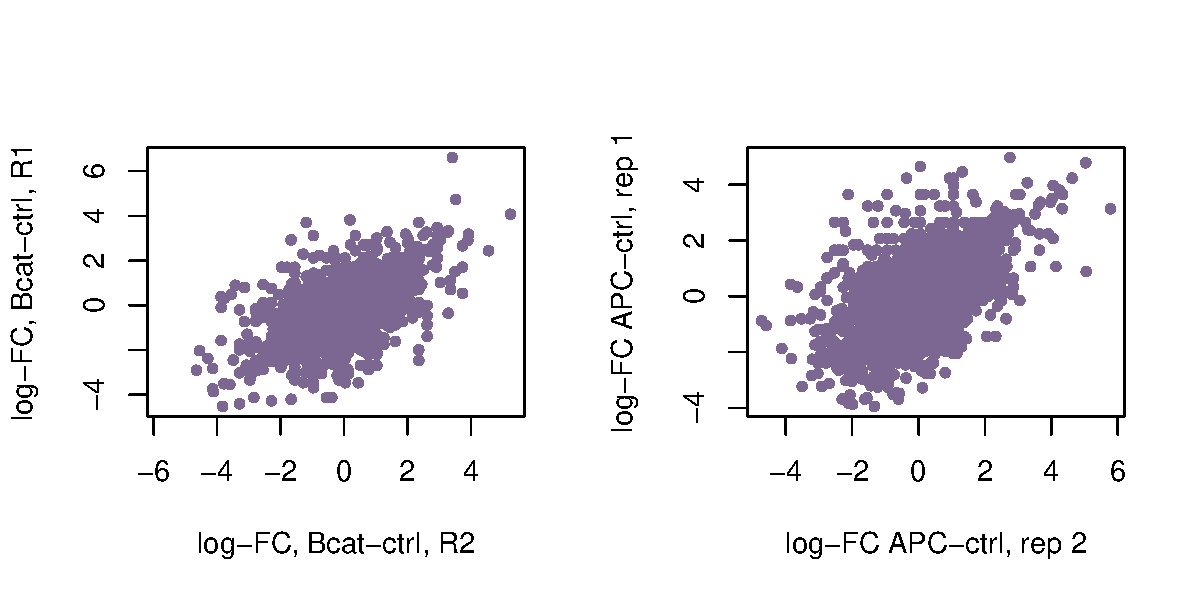
\includegraphics[width=\maxwidth]{figure/voomRepPlot} 

\end{knitrout}

Reproducibility of EVI and its fold changes with respect to the CTRL
\begin{knitrout}
\definecolor{shadecolor}{rgb}{0.969, 0.969, 0.969}\color{fgcolor}\begin{kframe}
\begin{alltt}
\hlkwd{par}\hlstd{(}\hlkwc{mfrow}\hlstd{=}\hlkwd{c}\hlstd{(}\hlnum{1}\hlstd{,}\hlnum{2}\hlstd{),} \hlkwc{cex}\hlstd{=}\hlnum{1.2}\hlstd{)}
\hlkwd{plot}\hlstd{(cpmDlog[,}\hlstr{"EVI_1"}\hlstd{]}\hlopt{-}\hlstd{cpmDlog[,}\hlstr{"CTRL_1"}\hlstd{],}
     \hlstd{cpmDlog[,}\hlstr{"EVI_2"}\hlstd{]}\hlopt{-}\hlstd{cpmDlog[,}\hlstr{"CTRL_2"}\hlstd{],}
     \hlkwc{ylab}\hlstd{=}\hlstr{"log-FC, EVI-ctrl, R1"}\hlstd{,}
     \hlkwc{xlab}\hlstd{=}\hlstr{"log-FC, EVI-ctrl, R2"}\hlstd{,}
     \hlkwc{pch}\hlstd{=}\hlnum{20}\hlstd{,} \hlkwc{col}\hlstd{=jpurp)}
\hlkwd{plot}\hlstd{(cpmDlog[,}\hlstr{"EVI_1"}\hlstd{], cpmDlog[,}\hlstr{"EVI_2"}\hlstd{],}
     \hlkwc{ylab}\hlstd{=}\hlstr{"log-cpm, EVI kd, R1"}\hlstd{,}
     \hlkwc{xlab}\hlstd{=}\hlstr{"log-cpm, EVI kd, R2"}\hlstd{,}
     \hlkwc{pch}\hlstd{=}\hlnum{20}\hlstd{,} \hlkwc{col}\hlstd{=jpurp)}
\end{alltt}
\end{kframe}
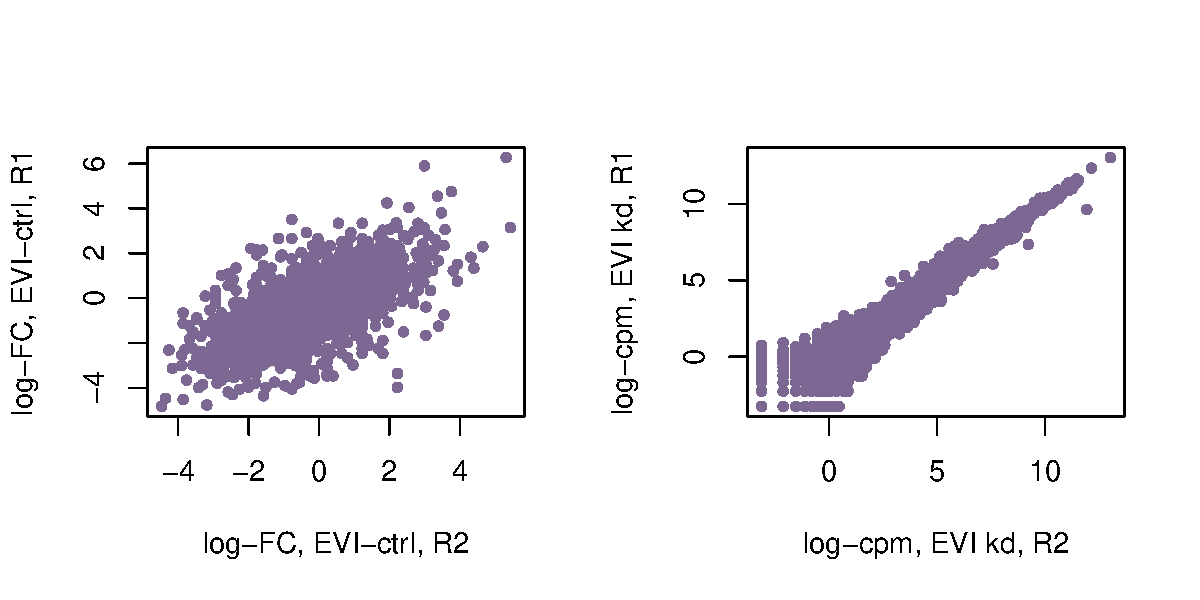
\includegraphics[width=\maxwidth]{figure/voomRepEVI} 

\end{knitrout}





Plot the siRNA efficiencies observed in the data
\begin{knitrout}
\definecolor{shadecolor}{rgb}{0.969, 0.969, 0.969}\color{fgcolor}\begin{kframe}
\begin{alltt}
\hlstd{knockdown} \hlkwb{<-} \hlkwd{c}\hlstd{(}\hlstr{"CTNNB1"}\hlstd{,} \hlstr{"EVI"}\hlstd{,} \hlstr{"APC"}\hlstd{,} \hlstr{"TCF7L2"}\hlstd{)}
\hlstd{geneTarget} \hlkwb{<-} \hlkwd{c}\hlstd{(}\hlstr{"CTNNB1"}\hlstd{,} \hlstr{"WLS"}\hlstd{,} \hlstr{"APC"}\hlstd{,} \hlstr{"TCF7L2"}\hlstd{)} \hlcom{### WLS is the EVI genen symbol}
\hlstd{genePick} \hlkwb{<-} \hlkwd{c}\hlstd{(geneTarget,}\hlstr{"AXIN2"}\hlstd{,} \hlstr{"ACTB"}\hlstd{)}
\hlstd{postProbDE[genePick, knockdown]}
\end{alltt}
\begin{verbatim}
##         Contrasts
##             CTNNB1       EVI      APC    TCF7L2
##   CTNNB1 1.0000000 0.0108482 0.026336 0.0003116
##   WLS    0.9093016 0.9999991 0.001961 0.0397116
##   APC    0.0009051 0.5449705 0.999917 0.9853499
##   TCF7L2 0.9997415 0.5592880 0.998739 0.9999973
##   AXIN2  0.9986680 0.9897556 0.999897 0.0019609
##   ACTB   0.0015294 0.0005056 0.323049 0.0074923
\end{verbatim}
\begin{alltt}
\hlstd{knockEff} \hlkwb{<-} \hlkwd{topTable}\hlstd{(subJlim[[}\hlnum{1}\hlstd{]],} \hlkwc{adjust}\hlstd{=}\hlstr{"BH"}\hlstd{,}
                     \hlkwc{n}\hlstd{=}\hlkwd{length}\hlstd{(postProbDE[,}\hlnum{1}\hlstd{]))[genePick,]}
\hlstd{knockNames} \hlkwb{<-} \hlkwd{paste0}\hlstd{(knockdown,}\hlstr{"."}\hlstd{,}\hlstr{"CTRL"}\hlstd{)}
\hlstd{knockObs} \hlkwb{<-} \hlkwd{cbind}\hlstd{(geneTarget, knockNames)}
\hlstd{knockPlot} \hlkwb{<-} \hlkwd{c}\hlstd{(}\hlnum{1}\hlstd{,}\hlnum{2}\hlopt{^}\hlkwd{as.numeric}\hlstd{(knockEff[knockObs]))}
\hlstd{postProbDE[geneTarget,]}
\end{alltt}
\begin{verbatim}
##         Contrasts
##               APC     AXIN1      BCL9    CTNNB1     EVI    TCF7L2
##   CTNNB1 0.026336 0.0020398 0.0082530 1.0000000 0.01085 0.0003116
##   WLS    0.001961 0.0032370 0.0004244 0.9093016 1.00000 0.0397116
##   APC    0.999917 0.0017990 0.0019270 0.0009051 0.54497 0.9853499
##   TCF7L2 0.998739 0.0003446 0.9978946 0.9997415 0.55929 0.9999973
\end{verbatim}
\begin{alltt}
\hlcom{## effectively the posterio probabilities are estimated as being all 1}
\hlkwd{topTable}\hlstd{(subJlim[[}\hlnum{1}\hlstd{]],} \hlkwc{coef}\hlstd{=}\hlnum{4}\hlstd{,} \hlkwc{adjust}\hlstd{=}\hlstr{"BH"}\hlstd{,} \hlkwc{n}\hlstd{=}\hlnum{3}\hlstd{)}
\end{alltt}
\begin{verbatim}
##         logFC AveExpr      t   P.Value adj.P.Val     B
## CTNNB1 -3.981   9.034 -30.95 7.343e-14 9.212e-10 20.80
## PDE4B  -2.047   8.095 -25.91 7.671e-13 4.812e-09 18.79
## KITLG  -2.876  10.581 -24.25 1.830e-12 7.652e-09 18.14
\end{verbatim}
\begin{alltt}
\hlcom{## coef=4 corresponds to "CTNNB1" knockdown, and actually it comes top in the effects}
\hlstd{BetaCatRank} \hlkwb{<-} \hlkwd{topTable}\hlstd{(subJlim[[}\hlnum{1}\hlstd{]],} \hlkwc{coef}\hlstd{=}\hlnum{4}\hlstd{,} \hlkwc{adjust}\hlstd{=}\hlstr{"BH"}\hlstd{,}
                        \hlkwc{n}\hlstd{=}\hlkwd{length}\hlstd{(postProbDE[,}\hlnum{1}\hlstd{]))}
\hlstd{BetaCatRank[}\hlkwd{which}\hlstd{(BetaCatRank}\hlopt{$}\hlstd{ID} \hlopt \hlstd{genePick),]}
\end{alltt}
\begin{verbatim}
## [1] logFC     AveExpr   t         P.Value   adj.P.Val B        
## <0 rows> (or 0-length row.names)
\end{verbatim}
\end{kframe}
\end{knitrout}

\begin{figure}[htbp]
\begin{center}
vspace{-3ex}
\begin{knitrout}
\definecolor{shadecolor}{rgb}{0.969, 0.969, 0.969}\color{fgcolor}\begin{kframe}
\begin{alltt}
\hlkwd{par}\hlstd{(}\hlkwc{cex}\hlstd{=}\hlnum{1.2}\hlstd{)}
\hlkwd{barplot}\hlstd{(knockPlot,} \hlkwc{width}\hlstd{=}\hlnum{.2}\hlstd{,} \hlkwc{space}\hlstd{=}\hlnum{2}\hlstd{,} \hlkwc{names.arg}\hlstd{=}\hlkwd{c}\hlstd{(}\hlstr{"CTRL"}\hlstd{,knockdown),}
        \hlkwc{xlim}\hlstd{=}\hlkwd{c}\hlstd{(}\hlnum{0}\hlstd{,}\hlnum{3}\hlstd{),} \hlkwc{cex.axis}\hlstd{=}\hlnum{1.1}\hlstd{,} \hlkwc{axis.lty}\hlstd{=}\hlnum{1}\hlstd{,} \hlkwc{ylab}\hlstd{=}\hlstr{"knockdown efficiencies"}\hlstd{,}
        \hlkwc{col}\hlstd{=jpurp)}
\end{alltt}
\end{kframe}
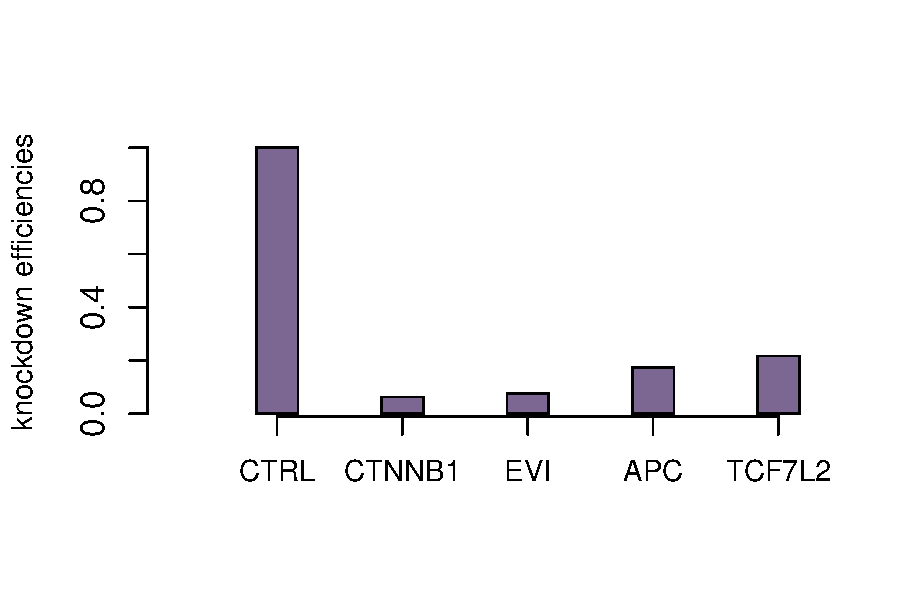
\includegraphics[width=\maxwidth]{figure/Efficiency_barplot} 

\end{knitrout}
\caption{The posterior probabilities of the knockdown targets being differentially expressed are effectively estimated all as being 1.}
\end{center}
\end{figure}

Plot effects observed in the data on typical wnt targets
\begin{knitrout}
\definecolor{shadecolor}{rgb}{0.969, 0.969, 0.969}\color{fgcolor}\begin{kframe}
\begin{alltt}
\hlcom{# moreBetaTargets <- c("MET", "EDN1", "HES1", "LAMC2", "PLAU", "SP5")}
\hlstd{knockdown} \hlkwb{<-} \hlkwd{c}\hlstd{(}\hlstr{"CTNNB1"}\hlstd{,} \hlstr{"EVI"}\hlstd{,} \hlstr{"APC"}\hlstd{,} \hlstr{"TCF7L2"}\hlstd{)}
\hlstd{wntTargets} \hlkwb{<-} \hlkwd{c}\hlstd{(}\hlstr{"AXIN2"}\hlstd{,} \hlstr{"RUNX2"}\hlstd{,} \hlstr{"SMAD7"}\hlstd{)}
\hlstd{postProbDE[wntTargets, knockdown]}
\end{alltt}
\begin{verbatim}
##        Contrasts
##          CTNNB1    EVI    APC   TCF7L2
##   AXIN2 0.99867 0.9898 0.9999 0.001961
##   RUNX2 0.02812 0.1168 0.1843 0.999737
##   SMAD7 0.38008 0.5950 0.7904 0.000694
\end{verbatim}
\begin{alltt}
\hlstd{wntEff} \hlkwb{<-} \hlkwd{topTable}\hlstd{(subJlim[[}\hlnum{1}\hlstd{]],} \hlkwc{adjust}\hlstd{=}\hlstr{"BH"}\hlstd{,}
                     \hlkwc{n}\hlstd{=}\hlkwd{length}\hlstd{(postProbDE[,}\hlnum{1}\hlstd{]))[wntTargets,]}
\hlstd{knockNames} \hlkwb{<-} \hlkwd{paste0}\hlstd{(knockdown,}\hlstr{"."}\hlstd{,}\hlstr{"CTRL"}\hlstd{)}
\hlstd{wntObs} \hlkwb{<-} \hlkwd{cbind}\hlstd{(}\hlkwd{rep}\hlstd{(wntTargets,} \hlkwc{each}\hlstd{=}\hlkwd{length}\hlstd{(knockdown)),}
                \hlkwd{rep}\hlstd{(knockNames,} \hlkwd{length}\hlstd{(wntTargets)) )}
\hlcom{# knockCol <- rainbow(length(knockdown), start=.6, end=1, alpha = .4)}
\hlstd{knockCol} \hlkwb{<-} \hlkwd{rgb}\hlstd{(r,g,b)}
\hlkwd{names}\hlstd{(knockCol)} \hlkwb{<-} \hlstd{knockdown}
\end{alltt}
\end{kframe}
\end{knitrout}

\begin{figure}[htbp]
\begin{center}
\begin{knitrout}
\definecolor{shadecolor}{rgb}{0.969, 0.969, 0.969}\color{fgcolor}\begin{kframe}
\begin{alltt}
\hlkwd{layout}\hlstd{(}\hlkwd{matrix}\hlstd{(}\hlkwd{c}\hlstd{(}\hlnum{1}\hlstd{,}\hlnum{2}\hlstd{)),} \hlkwc{heights}\hlstd{=}\hlkwd{c}\hlstd{(}\hlnum{1}\hlstd{,}\hlnum{3}\hlstd{))}
\hlkwd{par}\hlstd{(}\hlkwc{mar} \hlstd{=} \hlkwd{c}\hlstd{(}\hlnum{1}\hlstd{,}\hlnum{4}\hlstd{,}\hlnum{2}\hlstd{,}\hlnum{4}\hlstd{),} \hlkwc{cex}\hlstd{=}\hlnum{1.5}\hlstd{)}
\hlstd{mid_bar} \hlkwb{<-} \hlkwd{barplot}\hlstd{(}\hlkwd{t}\hlstd{(postProbDE[wntTargets, knockdown]),}
        \hlkwc{width}\hlstd{=}\hlnum{.1}\hlstd{,} \hlkwc{space}\hlstd{=}\hlkwd{c}\hlstd{(}\hlnum{4}\hlstd{,}\hlnum{14}\hlstd{),} \hlkwc{beside}\hlstd{=}\hlnum{TRUE}\hlstd{,}
        \hlkwc{col}\hlstd{=}\hlstr{"white"}\hlstd{,} \hlkwc{xlim}\hlstd{=}\hlkwd{c}\hlstd{(}\hlnum{0}\hlstd{,}\hlnum{11}\hlstd{),}
        \hlkwc{legend.text}\hlstd{=knockdown,}
        \hlkwc{args.legend}\hlstd{=}\hlkwd{list}\hlstd{(}\hlkwc{x}\hlstd{=}\hlnum{12}\hlstd{,} \hlkwc{y}\hlstd{=}\hlnum{.9}\hlstd{,} \hlkwc{fill}\hlstd{=knockCol,} \hlkwc{bty}\hlstd{=}\hlstr{"n"}\hlstd{),}
        \hlkwc{ylab}\hlstd{=}\hlstr{"pp DE"}\hlstd{,}
        \hlkwc{border}\hlstd{=}\hlnum{NA}\hlstd{,} \hlkwc{xaxt}\hlstd{=}\hlstr{"n"}\hlstd{)}
\hlkwd{segments}\hlstd{(}\hlkwd{as.vector}\hlstd{(mid_bar)}\hlopt{-}\hlnum{.2}\hlstd{,} \hlkwd{rep}\hlstd{(}\hlnum{0}\hlstd{,} \hlkwd{length}\hlstd{(mid_bar)),}
         \hlkwd{as.vector}\hlstd{(mid_bar)}\hlopt{-}\hlnum{.2}\hlstd{,} \hlkwd{as.vector}\hlstd{(}\hlkwd{t}\hlstd{(postProbDE[wntTargets, knockdown])),}
         \hlkwc{col}\hlstd{=knockCol,} \hlkwc{lwd}\hlstd{=}\hlnum{5}\hlstd{,} \hlkwc{lend}\hlstd{=}\hlnum{2}\hlstd{)}
\hlcom{# abline(h=.5, col=rgb(1, .4, 0), lwd=2, lty=2)}
\hlkwd{segments}\hlstd{(}\hlopt{-}\hlnum{1}\hlstd{,} \hlnum{.5}\hlstd{,} \hlnum{9}\hlstd{,} \hlnum{.5}\hlstd{,} \hlkwc{lwd}\hlstd{=}\hlnum{2}\hlstd{,} \hlkwc{lty}\hlstd{=}\hlnum{2}\hlstd{,} \hlkwc{col}\hlstd{=}\hlkwd{rgb}\hlstd{(}\hlnum{1}\hlstd{,} \hlnum{.4}\hlstd{,} \hlnum{0}\hlstd{))}
\hlkwd{abline}\hlstd{(}\hlkwc{h}\hlstd{=}\hlnum{0}\hlstd{)}
\hlkwd{par}\hlstd{(}\hlkwc{mar} \hlstd{=} \hlkwd{c}\hlstd{(}\hlnum{4}\hlstd{,}\hlnum{4}\hlstd{,}\hlnum{1}\hlstd{,}\hlnum{4}\hlstd{))}
\hlkwd{barplot}\hlstd{(}\hlkwd{t}\hlstd{(}\hlkwd{as.matrix}\hlstd{(wntEff[,knockNames])),}
        \hlkwc{width}\hlstd{=}\hlnum{.5}\hlstd{,} \hlkwc{space}\hlstd{=}\hlkwd{c}\hlstd{(}\hlnum{0}\hlstd{,}\hlnum{2}\hlstd{),} \hlkwc{beside}\hlstd{=}\hlnum{TRUE}\hlstd{,}
        \hlkwc{col}\hlstd{=knockCol,} \hlkwc{xlim}\hlstd{=}\hlkwd{c}\hlstd{(}\hlnum{0}\hlstd{,}\hlnum{11}\hlstd{),} \hlkwc{xpd}\hlstd{=}\hlnum{FALSE}\hlstd{,}
        \hlkwc{ylab}\hlstd{=}\hlstr{"Log Fold Change"}\hlstd{,}
\hlcom{#        legend.text=knockdown, }
\hlcom{#        args.legend=list(x=17, y=-1, fill=knockCol, bty="n"),}
        \hlkwc{names.arg}\hlstd{=wntTargets)}
\hlkwd{abline}\hlstd{(}\hlkwc{h}\hlstd{=}\hlnum{0}\hlstd{)}
\end{alltt}
\end{kframe}
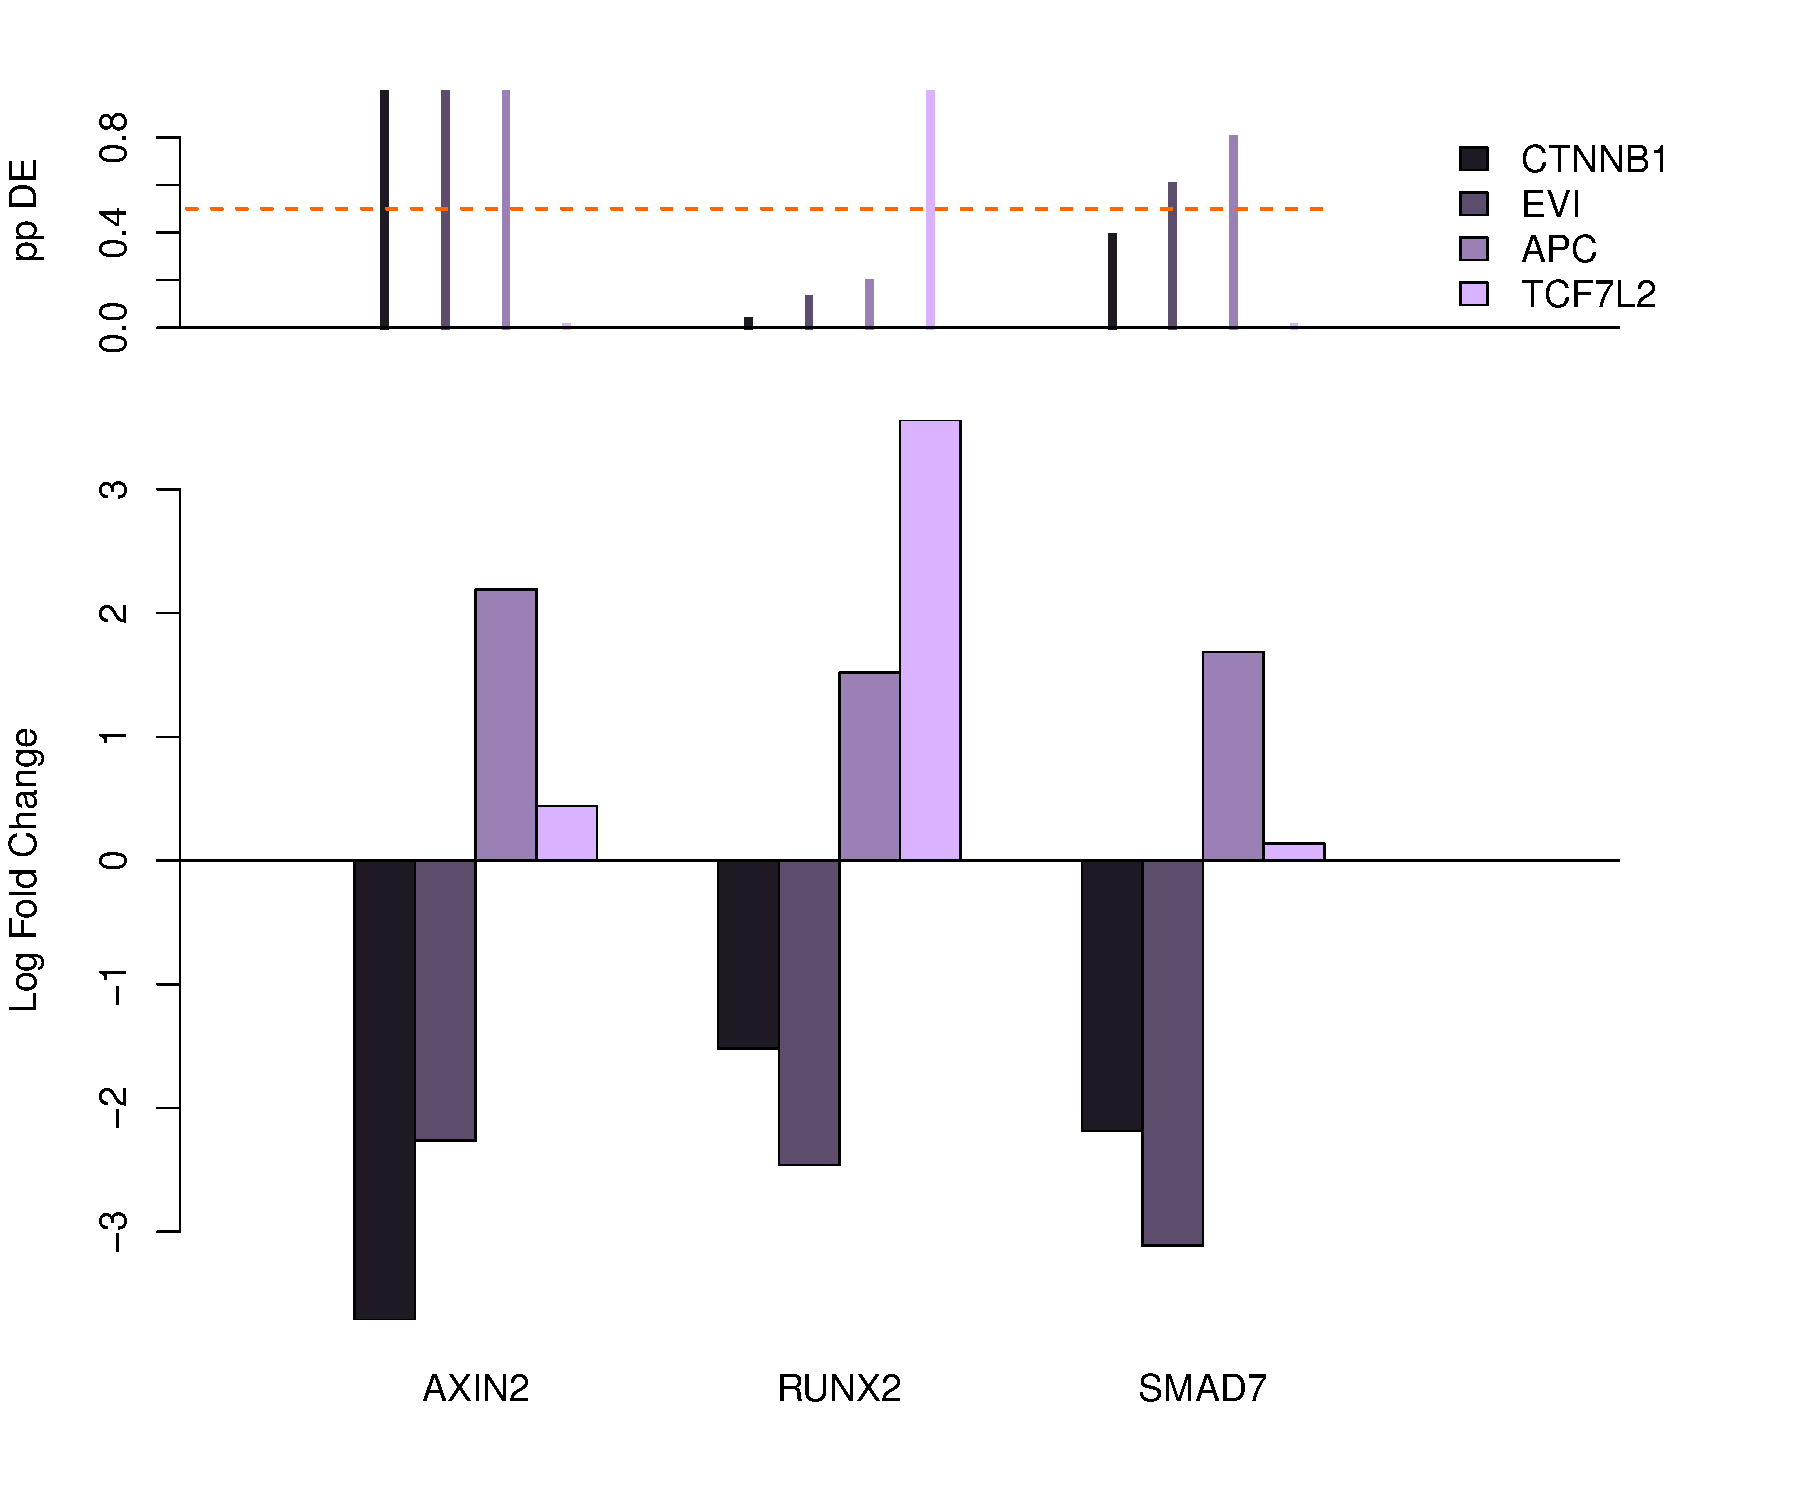
\includegraphics[width=\maxwidth]{figure/wntTargets} 

\end{knitrout}
\caption{Fold changes observed on well known typical wnt targets and their posterior probability of differential expression.}
\end{center}
\end{figure}
%\clearpage

\begin{knitrout}
\definecolor{shadecolor}{rgb}{0.969, 0.969, 0.969}\color{fgcolor}\begin{kframe}
\begin{alltt}
\hlcom{# global chunk options}
\hlstd{opts_chunk}\hlopt{$}\hlkwd{set}\hlstd{(}\hlkwc{cache} \hlstd{=} \hlnum{FALSE}\hlstd{,} \hlkwc{autodep} \hlstd{=} \hlnum{TRUE}\hlstd{)}
\end{alltt}
\end{kframe}
\end{knitrout}

\subsubsection*{Define models and classes}
Define a function building the nem models and the topology classes to consider, it defines the node names, enumerates all the models and selects those satisfying the desired contraints encoded by \verb'rnaiDisc'.
\begin{knitrout}
\definecolor{shadecolor}{rgb}{0.969, 0.969, 0.969}\color{fgcolor}\begin{kframe}
\begin{alltt}
\hlstd{buildTopologyClasses} \hlkwb{<-} \hlkwa{function}\hlstd{(}\hlkwc{postPde}\hlstd{,} \hlkwc{iOut}\hlstd{,} \hlkwc{iDisc}\hlstd{) \{}
    \hlcom{# Define node names corresponding to the knockdowns to model and select}
    \hlcom{# corresponding data}
    \hlstd{nodeNames} \hlkwb{<-} \hlkwd{unique}\hlstd{(}\hlkwd{colnames}\hlstd{(postPde)[}\hlkwd{which}\hlstd{(}\hlopt{!}\hlkwd{colnames}\hlstd{(postPde)} \hlopt \hlstd{iOut)])}
    \hlstd{postPde} \hlkwb{<-} \hlstd{postPde[,} \hlkwd{which}\hlstd{(}\hlkwd{colnames}\hlstd{(postPde)} \hlopt \hlstd{nodeNames)]}
    \hlstd{nNode} \hlkwb{<-} \hlkwd{length}\hlstd{(nodeNames)}
    \hlstd{nodeNames}

    \hlcom{### Enumerate all models}
    \hlstd{StdMods} \hlkwb{<-} \hlkwd{enumerate.models}\hlstd{(nodeNames,} \hlkwc{verbose} \hlstd{=} \hlnum{TRUE}\hlstd{)}
    \hlstd{numbStd} \hlkwb{<-} \hlkwd{length}\hlstd{(StdMods)}
    \hlstd{StdModels} \hlkwb{<-} \hlkwd{list}\hlstd{(}\hlkwc{AdjMats} \hlstd{= StdMods,} \hlkwc{numb} \hlstd{= numbStd,} \hlkwc{Names} \hlstd{= nodeNames)}

    \hlcom{### Define the set of constrained models, with no links between given nodes}
    \hlcom{### (for example ``EVI, APC'' on one side and ``CTNNB1, TCF7L2'' on the other)}
    \hlstd{E1} \hlkwb{<-} \hlkwd{which}\hlstd{(StdModels}\hlopt{$}\hlstd{Names} \hlopt \hlstd{iDisc)}
    \hlstd{E2} \hlkwb{<-} \hlkwd{which}\hlstd{(}\hlopt{!}\hlstd{StdModels}\hlopt{$}\hlstd{Names} \hlopt \hlstd{iDisc)}
    \hlstd{stdEl} \hlkwb{<-} \hlkwd{c}\hlstd{()}
    \hlcom{### A numerical vector with the indeces of the models satisfying the}
    \hlcom{### contraints}
    \hlkwa{for} \hlstd{(i} \hlkwa{in} \hlnum{1}\hlopt{:}\hlstd{StdModels}\hlopt{$}\hlstd{numb) \{}
        \hlkwa{if} \hlstd{(}\hlopt{!}\hlstd{(}\hlkwd{sum}\hlstd{(StdModels}\hlopt{$}\hlstd{AdjMats[[i]][E2, E1])} \hlopt{+} \hlkwd{sum}\hlstd{(StdModels}\hlopt{$}\hlstd{AdjMats[[i]][E1,}
            \hlstd{E2])))}
            \hlstd{stdEl} \hlkwb{<-} \hlkwd{c}\hlstd{(stdEl, i)}
    \hlstd{\}}
    \hlkwd{list}\hlstd{(}\hlkwc{allModels} \hlstd{= StdModels,} \hlkwc{constModels} \hlstd{= stdEl,} \hlkwc{selData} \hlstd{= postPde)}
\hlstd{\}}
\end{alltt}
\end{kframe}
\end{knitrout}

\subsubsection*{Evaluate Bayes factors between selected models}
Define a function evaluating the Bayes factors for the selected data according to the definition in equation \eqref{eq:classBF}, between the classes of topologies corresponding to the activation by sensitization and the direct activation models. When considering \emph{EVI, APC, CTBNN1} and \emph{TCF7L2} for example no links are allowed in the direct activation model between the subnets including the pairs \emph{EVI, APC} and \emph{CTBNN1, TCF7L2} respectively.
Bayes factors are calculated between a topology class and its complement, rather than between classes included in each other, as the cut-off for the probability of a downstream effect (or differential expression) increases, in a continuous data approach.
\begin{knitrout}
\definecolor{shadecolor}{rgb}{0.969, 0.969, 0.969}\color{fgcolor}\begin{kframe}
\begin{alltt}
\hlstd{dataBFtopologyClasses} \hlkwb{<-} \hlkwa{function}\hlstd{(}\hlkwc{postPde}\hlstd{,} \hlkwc{allModels}\hlstd{,} \hlkwc{constModels}\hlstd{) \{}
    \hlcom{### Define some working variables}
    \hlstd{myp} \hlkwb{<-} \hlkwd{seq}\hlstd{(}\hlnum{0.01}\hlstd{,} \hlnum{0.99}\hlstd{,} \hlnum{0.01}\hlstd{)}
    \hlcom{# posterior probability cut-off for differential expression}
    \hlstd{listScores} \hlkwb{<-} \hlkwd{list}\hlstd{()}  \hlcom{# all scores}
    \hlstd{subScores} \hlkwb{<-} \hlkwd{list}\hlstd{()}  \hlcom{# scores of constrained models, a subset of the whole set}
    \hlstd{nG} \hlkwb{<-} \hlkwd{c}\hlstd{()}  \hlcom{# number of genes selected for each cut-off}
    \hlstd{vecBF} \hlkwb{<-} \hlkwd{c}\hlstd{()}

    \hlkwa{for} \hlstd{(tmpp} \hlkwa{in} \hlstd{myp) \{}
        \hlstd{tmp_sel} \hlkwb{<-} \hlkwd{which}\hlstd{(}\hlkwd{apply}\hlstd{(postPde} \hlopt{>} \hlstd{tmpp,} \hlnum{1}\hlstd{, any))}
        \hlstd{D_sel} \hlkwb{<-} \hlstd{postPde[tmp_sel, ]}
        \hlstd{nG} \hlkwb{<-} \hlkwd{c}\hlstd{(nG,} \hlkwd{dim}\hlstd{(D_sel)[}\hlnum{1}\hlstd{])}
        \hlstd{tmpScore} \hlkwb{<-} \hlkwd{sapply}\hlstd{(allModels}\hlopt{$}\hlstd{AdjMats, netScore, D_sel)}
        \hlstd{listScores} \hlkwb{<-} \hlkwd{c}\hlstd{(listScores,} \hlkwd{list}\hlstd{(tmpScore))}
        \hlstd{tmpSub} \hlkwb{<-} \hlstd{tmpScore[constModels]}
        \hlstd{subScores} \hlkwb{<-} \hlkwd{c}\hlstd{(subScores,} \hlkwd{list}\hlstd{(tmpSub))}
        \hlstd{vecBF} \hlkwb{<-} \hlkwd{c}\hlstd{(vecBF,} \hlkwd{fullSimpleBF}\hlstd{(tmpScore[}\hlopt{-}\hlstd{constModels], tmpSub))}
    \hlstd{\}}
    \hlstd{matBF} \hlkwb{<-} \hlkwd{matrix}\hlstd{(vecBF,} \hlkwc{ncol} \hlstd{=} \hlnum{2}\hlstd{,} \hlkwc{byrow} \hlstd{= T)}
    \hlstd{matBF} \hlkwb{<-} \hlkwd{cbind}\hlstd{(matBF, myp)}
    \hlkwd{colnames}\hlstd{(matBF)} \hlkwb{<-} \hlkwd{c}\hlstd{(}\hlstr{"logBF"}\hlstd{,} \hlstr{"BF"}\hlstd{,} \hlstr{"podd"}\hlstd{)}
    \hlkwd{list}\hlstd{(}\hlkwc{allScores} \hlstd{= listScores,} \hlkwc{constScores} \hlstd{= subScores,} \hlkwc{BayesFactors} \hlstd{= matBF,}
        \hlkwc{nSelGenes} \hlstd{= nG,} \hlkwc{cutoffP} \hlstd{= myp)}
\hlstd{\}}
\end{alltt}
\end{kframe}
\end{knitrout}

%opts_chunk$set(echo=FALSE) %%% causes problems with alignment
\subsection*{Selection of knockdown experiments modelled in the analysis}
The nem analysis is performed including 4 knockdown experiments in the modelling, namely EVI, APC, TCF7L2 and CTNNB1.

\begin{knitrout}
\definecolor{shadecolor}{rgb}{0.969, 0.969, 0.969}\color{fgcolor}\begin{kframe}
\begin{alltt}
\hlkwd{library}\hlstd{(nem)}
\hlstd{rnaiOut} \hlkwb{<-} \hlkwd{c}\hlstd{(}\hlstr{"AXIN1"}\hlstd{,} \hlstr{"BCL9"}\hlstd{,} \hlstr{"CTRL"}\hlstd{)}
\hlcom{## set of rnai to leave out}
\hlstd{rnaiDisc} \hlkwb{<-} \hlkwd{c}\hlstd{(}\hlstr{"EVI"}\hlstd{,} \hlstr{"APC"}\hlstd{)}
\hlcom{## set of rnai assumed disconnected from the others (CTNNB1 and TCF7L2)}
\end{alltt}
\end{kframe}
\end{knitrout}

\subsubsection*{NEM analysis}
Perform nem analysis and evaluate Bayes factors
\begin{knitrout}
\definecolor{shadecolor}{rgb}{0.969, 0.969, 0.969}\color{fgcolor}\begin{kframe}
\begin{alltt}
\hlstd{topClasses} \hlkwb{<-} \hlkwd{buildTopologyClasses}\hlstd{(subJodd, rnaiOut, rnaiDisc)}
\end{alltt}
\begin{verbatim}
## Generated 355 unique models ( out of 4096 )
\end{verbatim}
\begin{alltt}
\hlstd{topClassBF} \hlkwb{<-} \hlkwd{dataBFtopologyClasses}\hlstd{(topClasses}\hlopt{$}\hlstd{selData,}
                                    \hlstd{topClasses}\hlopt{$}\hlstd{allModels,}
                                    \hlstd{topClasses}\hlopt{$}\hlstd{constModels)}
\end{alltt}
\end{kframe}
\end{knitrout}

\subsubsection*{Plot Bayes factors}
Plot the log Bayes factors between the two classes of topologies corresponding to activation by sensitization and direct activation model as a function of the cut-off posterior probabilities of differential expression.
\begin{knitrout}
\definecolor{shadecolor}{rgb}{0.969, 0.969, 0.969}\color{fgcolor}\begin{kframe}
\begin{alltt}
\hlkwd{library}\hlstd{(plotrix)}
\hlstd{matBFplot} \hlkwb{<-} \hlstd{topClassBF}\hlopt{$}\hlstd{BayesFactors[,} \hlnum{1}\hlstd{]}
\hlstd{matBFplot} \hlkwb{<-} \hlstd{topClassBF}\hlopt{$}\hlstd{BayesFactors[,} \hlnum{1}\hlstd{]}
\hlstd{biggerHalf} \hlkwb{<-} \hlkwd{which}\hlstd{(topClassBF}\hlopt{$}\hlstd{cutoffP} \hlopt{>} \hlnum{0.485}\hlstd{)}
\hlstd{matBFplot} \hlkwb{<-} \hlstd{topClassBF}\hlopt{$}\hlstd{BayesFactors[biggerHalf,} \hlnum{1}\hlstd{]}
\hlstd{cutsPlot} \hlkwb{<-} \hlstd{topClassBF}\hlopt{$}\hlstd{cutoffP[biggerHalf]}
\end{alltt}
\end{kframe}
\end{knitrout}

\begin{figure}[htbp]
\begin{center}
\begin{knitrout}
\definecolor{shadecolor}{rgb}{0.969, 0.969, 0.969}\color{fgcolor}\begin{kframe}
\begin{alltt}
\hlkwd{par}\hlstd{(}\hlkwc{cex.lab}\hlstd{=}\hlnum{1.4}\hlstd{,} \hlkwc{cex.axis}\hlstd{=}\hlnum{1.1}\hlstd{)}
\hlkwd{plot}\hlstd{(cutsPlot, matBFplot,} \hlkwc{type}\hlstd{=}\hlstr{"l"}\hlstd{,} \hlkwc{col}\hlstd{=}\hlnum{4}\hlstd{,} \hlkwc{lwd}\hlstd{=}\hlnum{3}\hlstd{,}
\hlkwc{ylab}\hlstd{=}\hlstr{"log Bayes Factor"}\hlstd{,} \hlkwc{xlab}\hlstd{=}\hlstr{"Probability cutoff for downstream effects"}\hlstd{,}
\hlkwc{xaxt}\hlstd{=}\hlstr{"n"}\hlstd{,} \hlkwc{yaxt}\hlstd{=}\hlstr{"n"}\hlstd{,} \hlkwc{ylim}\hlstd{=}\hlkwd{extendrange}\hlstd{(}\hlkwc{r}\hlstd{=}\hlkwd{range}\hlstd{(matBFplot),} \hlkwc{f}\hlstd{=}\hlnum{.1}\hlstd{))}
\hlstd{ticks2} \hlkwb{<-} \hlkwd{axTicks}\hlstd{(}\hlnum{2}\hlstd{); ticks2} \hlkwb{<-} \hlstd{ticks2[}\hlkwd{which}\hlstd{(ticks2}\hlopt{>=}\hlnum{0}\hlstd{)]}
\hlkwd{axis}\hlstd{(}\hlnum{2}\hlstd{,} \hlkwc{at}\hlstd{=}\hlkwd{c}\hlstd{(}\hlkwd{range}\hlstd{(matBFplot)[}\hlnum{1}\hlstd{],ticks2),}
\hlkwc{labels}\hlstd{=}\hlkwd{c}\hlstd{(}\hlkwd{round}\hlstd{(}\hlkwd{range}\hlstd{(matBFplot)[}\hlnum{1}\hlstd{],}\hlnum{2}\hlstd{),ticks2))}
\hlkwd{axis}\hlstd{(}\hlnum{1}\hlstd{,} \hlkwc{at}\hlstd{=topClassBF}\hlopt{$}\hlstd{cutoffP[}\hlkwd{which}\hlstd{(}\hlkwd{seq}\hlstd{(}\hlnum{1}\hlopt{:}\hlnum{100}\hlstd{)}\hlopt\hlnum{5} \hlopt{==} \hlnum{0}\hlstd{)],}
\hlkwc{labels}\hlstd{=topClassBF}\hlopt{$}\hlstd{cutoffP[}\hlkwd{which}\hlstd{(}\hlkwd{seq}\hlstd{(}\hlnum{1}\hlopt{:}\hlnum{100}\hlstd{)}\hlopt\hlnum{5} \hlopt{==} \hlnum{0}\hlstd{)])}
\hlkwd{axis}\hlstd{(}\hlnum{3}\hlstd{,} \hlkwc{at}\hlstd{=topClassBF}\hlopt{$}\hlstd{cutoffP[}\hlkwd{which}\hlstd{(}\hlkwd{seq}\hlstd{(}\hlnum{1}\hlopt{:}\hlnum{100}\hlstd{)}\hlopt\hlnum{5} \hlopt{==} \hlnum{0}\hlstd{)],}
\hlkwc{labels}\hlstd{=topClassBF}\hlopt{$}\hlstd{nSelGenes[}\hlkwd{which}\hlstd{(}\hlkwd{seq}\hlstd{(}\hlnum{1}\hlopt{:}\hlnum{100}\hlstd{)}\hlopt\hlnum{5} \hlopt{==} \hlnum{0}\hlstd{)])}
\hlkwd{mtext}\hlstd{(}\hlstr{"Number of Targets"}\hlstd{,} \hlkwc{side}\hlstd{=}\hlnum{3}\hlstd{,} \hlkwc{line}\hlstd{=}\hlnum{3}\hlstd{,} \hlkwc{cex}\hlstd{=}\hlnum{1.4}\hlstd{)} \hlcom{# margin text}
\hlkwd{abline}\hlstd{(}\hlkwc{h}\hlstd{=}\hlnum{0}\hlstd{,} \hlkwc{col}\hlstd{=}\hlstr{"firebrick3"}\hlstd{,} \hlkwc{lwd}\hlstd{=}\hlnum{4}\hlstd{)}
\hlkwd{abline}\hlstd{(}\hlkwc{v}\hlstd{=}\hlnum{0.95}\hlstd{,} \hlkwc{col}\hlstd{=}\hlstr{"goldenrod2"}\hlstd{,} \hlkwc{lwd}\hlstd{=}\hlnum{3}\hlstd{,} \hlkwc{lty}\hlstd{=}\hlnum{4}\hlstd{)}
\hlkwd{abline}\hlstd{(}\hlkwc{v}\hlstd{=topClassBF}\hlopt{$}\hlstd{cutoffP[}\hlkwd{min}\hlstd{(}\hlkwd{which}\hlstd{(topClassBF}\hlopt{$}\hlstd{BayesFactors[,}\hlnum{2}\hlstd{]}\hlopt{>}\hlnum{1}\hlstd{))],}
\hlkwc{col}\hlstd{=}\hlstr{"orchid3"}\hlstd{,} \hlkwc{lwd}\hlstd{=}\hlnum{3}\hlstd{,} \hlkwc{lty}\hlstd{=}\hlnum{4}\hlstd{)}
\hlkwd{text}\hlstd{(}\hlnum{.01}\hlstd{,}\hlnum{300}\hlstd{,} \hlkwc{pos}\hlstd{=}\hlnum{4}\hlstd{,} \hlkwc{labels}\hlstd{=}\hlstr{"Activation by Sensitization Model"}\hlstd{)}
\hlkwd{text}\hlstd{(}\hlnum{.01}\hlstd{,}\hlopt{-}\hlnum{300}\hlstd{,} \hlkwc{pos}\hlstd{=}\hlnum{4}\hlstd{,} \hlkwc{labels}\hlstd{=}\hlstr{"Direct Activation Model"}\hlstd{)}
\end{alltt}
\end{kframe}
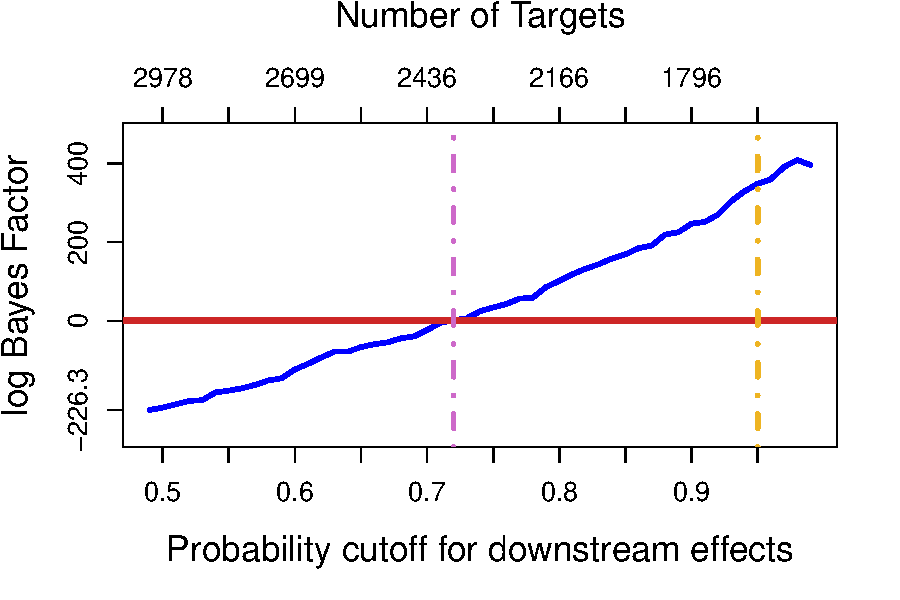
\includegraphics[width=\maxwidth]{figure/plotBF3} 

\end{knitrout}
\caption{The blue line shows log Bayes Factors (y-axis) between the class of topologies corresponding to activation by sensitization models to the class of topologies corresponding to direct activation models. Log Bayes Factors were obtained from nested effect models for different numbers of potential target genes (x-axis, top), which were included according to a cut-off on the posterior probability that a gene is affected for at least one perturbation (among those included in the model). Positive log Bayes factor reflect evidence in favour of the activation by sensitization model. Log Bayes Factors above 10 can be considered strong evidence. The dashed purple line indicates the smallest cutoff yielding a model that favours the activation by sensitization model. A conservative cutoff of 95\% posterior probability that an observed expression difference is a true response to perturbation is marked by the yellow dashed line.}
\label{fig:classBF}
\end{center}
\end{figure}

%\clearpage

\subsubsection*{Plot genes with highest posterior probability of differential expression in at least one intervention}
Visualize in a quilt plot the posterior probability of differential expression for the genes which have a posterior probability larger than .5 of showing an effect in at least one of the knockdown experiments included in the model, order by the minimum between the probabilities of differential expression in the knockdown of EVI, CTNNB1, TCF7L2 and the probability of no differential expression in the knockdown of APC.

\begin{knitrout}
\definecolor{shadecolor}{rgb}{0.969, 0.969, 0.969}\color{fgcolor}\begin{kframe}
\begin{alltt}
\hlkwd{library}\hlstd{(fields)}
\hlkwd{library}\hlstd{(RColorBrewer)}
\end{alltt}
\end{kframe}
\end{knitrout}


Gene ordering.
\begin{knitrout}
\definecolor{shadecolor}{rgb}{0.969, 0.969, 0.969}\color{fgcolor}\begin{kframe}
\begin{alltt}
\hlcom{# set of rnai's modelled}
\hlstd{subNet1} \hlkwb{<-} \hlkwd{c}\hlstd{(}\hlstr{"EVI"}\hlstd{,} \hlstr{"APC"}\hlstd{)}
\hlstd{subNet2} \hlkwb{<-} \hlkwd{c}\hlstd{(}\hlstr{"CTNNB1"}\hlstd{,} \hlstr{"TCF7L2"}\hlstd{)}
\hlstd{modelPde} \hlkwb{<-} \hlstd{topClasses}\hlopt{$}\hlstd{selData[,}\hlkwd{c}\hlstd{(subNet1, subNet2)]}
\hlstd{modelPde} \hlkwb{<-} \hlstd{modelPde[}\hlkwd{which}\hlstd{(}\hlkwd{apply}\hlstd{(modelPde}\hlopt{>}\hlnum{.5}\hlstd{,} \hlnum{1}\hlstd{, any )),]}
\hlstd{ordMatrix} \hlkwb{<-} \hlstd{modelPde}
\hlstd{ordMatrix[,}\hlstr{"APC"}\hlstd{]} \hlkwb{<-} \hlnum{1}\hlopt{-}\hlstd{ordMatrix[,}\hlstr{"APC"}\hlstd{]}
\hlstd{minProbDE} \hlkwb{<-} \hlkwd{apply}\hlstd{(ordMatrix,}\hlnum{1}\hlstd{,min)}
\hlstd{orderPs} \hlkwb{<-} \hlkwd{order}\hlstd{(minProbDE,} \hlkwc{decreasing}\hlstd{=}\hlnum{TRUE}\hlstd{)}
\hlstd{nrcolors} \hlkwb{<-} \hlnum{100}
\hlstd{half} \hlkwb{<-} \hlnum{1}\hlopt{+}\hlstd{nrcolors}\hlopt{/}\hlnum{2}
\hlstd{colpal} \hlkwb{<-} \hlkwd{c}\hlstd{(}\hlkwd{brewer.pal}\hlstd{(}\hlnum{9}\hlstd{,} \hlstr{"Blues"}\hlstd{)[}\hlnum{9}\hlopt{:}\hlnum{1}\hlstd{],} \hlkwd{brewer.pal}\hlstd{(}\hlnum{9}\hlstd{,}\hlstr{"Reds"}\hlstd{)[}\hlnum{1}\hlopt{:}\hlnum{9}\hlstd{])}
\hlstd{colorpalette} \hlkwb{<-} \hlkwd{colorRampPalette}\hlstd{(colpal)(nrcolors)}
\hlstd{quantileBreaks} \hlkwb{<-} \hlkwd{c}\hlstd{(}\hlkwd{quantile}\hlstd{(postProbDE[}\hlkwd{which}\hlstd{(postProbDE} \hlopt{<} \hlnum{.5}\hlstd{)],}
                             \hlkwc{probs} \hlstd{=} \hlkwd{seq}\hlstd{(}\hlnum{0}\hlstd{,} \hlnum{1}\hlstd{,} \hlkwc{length} \hlstd{= half)),}
                    \hlkwd{quantile}\hlstd{(postProbDE[}\hlkwd{which}\hlstd{(postProbDE} \hlopt{>=} \hlnum{.5}\hlstd{)],}
                             \hlkwc{probs} \hlstd{=} \hlkwd{seq}\hlstd{(}\hlnum{0}\hlstd{,} \hlnum{1}\hlstd{,} \hlkwc{length} \hlstd{= half}\hlopt{-}\hlnum{1}\hlstd{)))}
\end{alltt}
\end{kframe}
\end{knitrout}

\begin{figure}[htbp]
\begin{center}
\begin{knitrout}
\definecolor{shadecolor}{rgb}{0.969, 0.969, 0.969}\color{fgcolor}\begin{kframe}
\begin{alltt}
\hlkwd{par}\hlstd{(} \hlkwc{mar} \hlstd{=} \hlkwd{par}\hlstd{(} \hlstr{"mar"} \hlstd{)} \hlopt{+} \hlkwd{c}\hlstd{(} \hlnum{0}\hlstd{,} \hlnum{2}\hlstd{,} \hlnum{0}\hlstd{,} \hlnum{4} \hlstd{) )}
\hlstd{imgOdd} \hlkwb{<-} \hlstd{modelPde[orderPs,}\hlkwd{rev}\hlstd{(knockdown)]}
\hlstd{sep} \hlkwb{<-} \hlnum{40}
\hlstd{sepLine} \hlkwb{<-} \hlkwd{matrix}\hlstd{(}\hlkwd{runif}\hlstd{(sep}\hlopt{*}\hlnum{4}\hlstd{),} \hlkwc{nrow}\hlstd{=sep,} \hlkwc{ncol}\hlstd{=}\hlnum{4}\hlstd{)}
\hlkwd{colnames}\hlstd{(sepLine)} \hlkwb{<-} \hlkwd{colnames}\hlstd{(imgOdd)} \hlcom{### check that the order is right!!!}
\hlstd{left} \hlkwb{<-} \hlnum{1}\hlopt{:}\hlnum{750}
\hlstd{imgLeft} \hlkwb{<-} \hlstd{imgOdd[left,]}
\hlstd{imgRight} \hlkwb{<-} \hlstd{imgOdd[}\hlopt{-}\hlstd{left,]}
\hlcom{# imgOdd <- rbind(sepLine, imgLeft, sepLine, imgRight)}
\hlstd{imgOdd} \hlkwb{<-} \hlkwd{rbind}\hlstd{(imgLeft, sepLine, imgRight)}
\hlstd{x} \hlkwb{<-} \hlnum{1}\hlopt{:}\hlkwd{nrow}\hlstd{(imgOdd)}
\hlstd{y} \hlkwb{<-} \hlnum{1}\hlopt{:}\hlkwd{ncol}\hlstd{(imgOdd)}
\hlkwd{image}\hlstd{(x,y,imgOdd,} \hlkwc{xaxt}\hlstd{=}\hlstr{"n"}\hlstd{,} \hlkwc{yaxt}\hlstd{=}\hlstr{"n"}\hlstd{,} \hlkwc{ylab}\hlstd{=}\hlstr{""}\hlstd{,} \hlkwc{xlab}\hlstd{=}\hlstr{""}\hlstd{,}
\hlkwc{col}\hlstd{=colorpalette,} \hlkwc{breaks}\hlstd{=quantileBreaks)}
\hlcom{# axis( 1, labels=c(1, nrow(imgOdd)-2*sep), at=seq(1,nrow(imgOdd),length.out=2))}
\hlkwd{axis}\hlstd{(} \hlnum{1}\hlstd{,} \hlkwc{labels}\hlstd{=}\hlkwd{c}\hlstd{(}\hlnum{1}\hlstd{,} \hlkwd{nrow}\hlstd{(imgOdd)}\hlopt{-}\hlstd{sep),} \hlkwc{at}\hlstd{=}\hlkwd{seq}\hlstd{(}\hlnum{1}\hlstd{,}\hlkwd{nrow}\hlstd{(imgOdd),}\hlkwc{length.out}\hlstd{=}\hlnum{2}\hlstd{))}
\hlkwd{axis}\hlstd{(} \hlnum{2}\hlstd{,} \hlkwc{at}\hlstd{=}\hlkwd{seq}\hlstd{(}\hlnum{1}\hlstd{,}\hlkwd{ncol}\hlstd{(imgOdd),}\hlkwc{length.out}\hlstd{=}\hlkwd{ncol}\hlstd{(imgOdd) ),}
\hlkwc{labels}\hlstd{=} \hlkwd{colnames}\hlstd{( imgOdd ),} \hlkwc{las}\hlstd{=} \hlnum{2} \hlstd{)}
\hlkwd{image.plot}\hlstd{(imgOdd,} \hlkwc{xaxt}\hlstd{=}\hlstr{"n"}\hlstd{,} \hlkwc{yaxt}\hlstd{=}\hlstr{"n"}\hlstd{,} \hlkwc{legend.only}\hlstd{=}\hlnum{TRUE}\hlstd{,}
\hlkwc{col}\hlstd{=colorpalette)}
\hlstd{colLine} \hlkwb{<-} \hlnum{751}\hlopt{:}\hlstd{(}\hlnum{750}\hlopt{+}\hlstd{sep)}
\hlkwa{for}\hlstd{(i} \hlkwa{in} \hlstd{colLine)} \hlkwd{abline}\hlstd{(}\hlkwc{v}\hlstd{=i,} \hlkwc{col}\hlstd{=}\hlkwd{rgb}\hlstd{(}\hlnum{.5}\hlstd{,}\hlnum{.9}\hlstd{,}\hlnum{0}\hlstd{))}
\end{alltt}
\end{kframe}
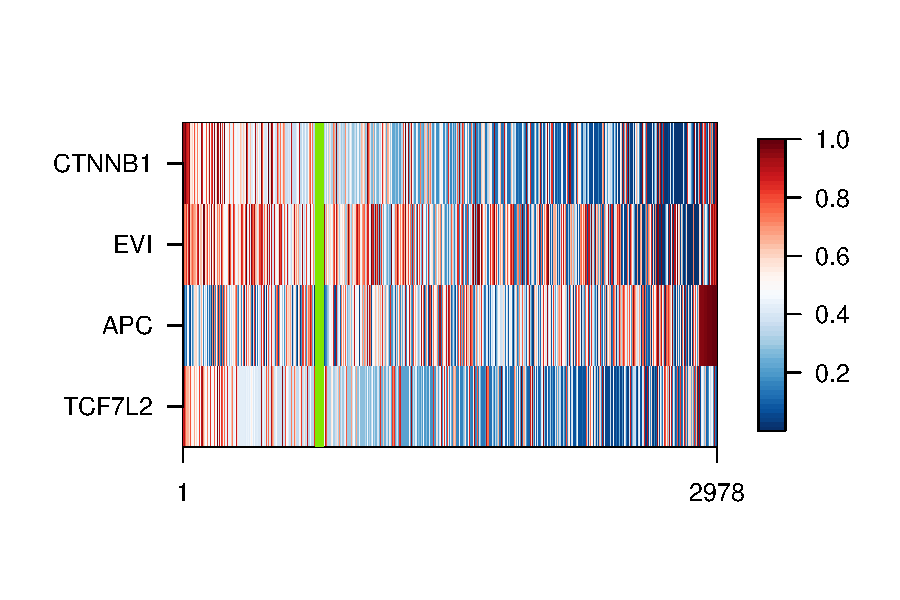
\includegraphics[width=\maxwidth]{figure/minPsRBgreen} 

\end{knitrout}
\caption{{\bf Posterior probabilities of differential expression.} Heatmap of the posterior probabilities of differential expression in the silencing experiments. Only genes which have a posterior probability larger than .5 of showing an effect in at least one of the knockdown experiments are shown. The green line leaves about 750 genes on its left. The pattern there shows that the majority of those genes respond not only to intervention on $\beta$-catenin, but also to EVI, while most of them do not respond to the APC.}
\label{fig:heatmap}
\end{center}
\end{figure}
%%%----------------------------------------------------------%%%

%%%--------- Input noConan tex ----------%%%
\newpage
\section*{No-Conan on RNAseq expression data from the Wnt pathway in colorectal cancer}
\input noConan.tex
%%%----------------------------------------------------------%%%

\clearpage
\bibliographystyle{plainnat}
\bibliography{WNTcrc}
\end{document}
